\begin{center}
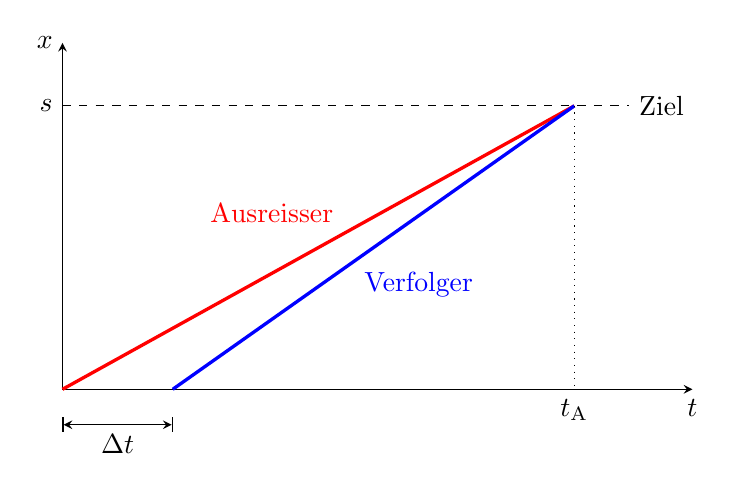
\begin{tikzpicture}[>=stealth]
 \draw[->] (0,0) -- (8,0) node[below] {$t$};
 \draw[->] (0,0) -- (0,4.4) node[left] {$x$};
 \draw[dashed] (0,3.6) node[left] {$s$} -- (7.2,3.6) node[right] {Ziel};
 \draw[red, very thick] (0,0) -- (6.5,3.6) node[pos=0.55, above left] {Ausreisser};
 \draw[blue, very thick] (1.4,0) -- (6.5,3.6) node[pos=0.45, below right] {Verfolger};
 \draw[|<->|] (0,-0.45) -- (1.4,-0.45) node[midway, below] {$\Delta t$};
 \draw[dotted] (6.5,3.6) -- (6.5,0) node[below] {$t_\mathrm{A}$};
\end{tikzpicture}
\end{center}

Die Zeit wird ab dem Moment gezählt, in dem der Ausreisser die Marke passiert, $x$ ist der Ort ab der Marke. Der Ausreisser braucht bis ins Ziel
\begin{align}
 t_\mathrm{A} &= \tAuF = \frac{\sV}{\vAu} = \tAu
\end{align}
Die Verfolger starten um $\Delta t$ später und müssen spätestens gleichzeitig im Ziel sein. Ihnen bleibt also die Zeit $t_\mathrm{A}-\Delta t$, und ihre Geschwindigkeit muss mindestens
\begin{align}
 v_\mathrm{V} &= \vVF \\
   &= \frac{\sV}{\tAu-\tV} = \vV \approx \result{\vVkP{0}{3}}
\end{align}
betragen.
